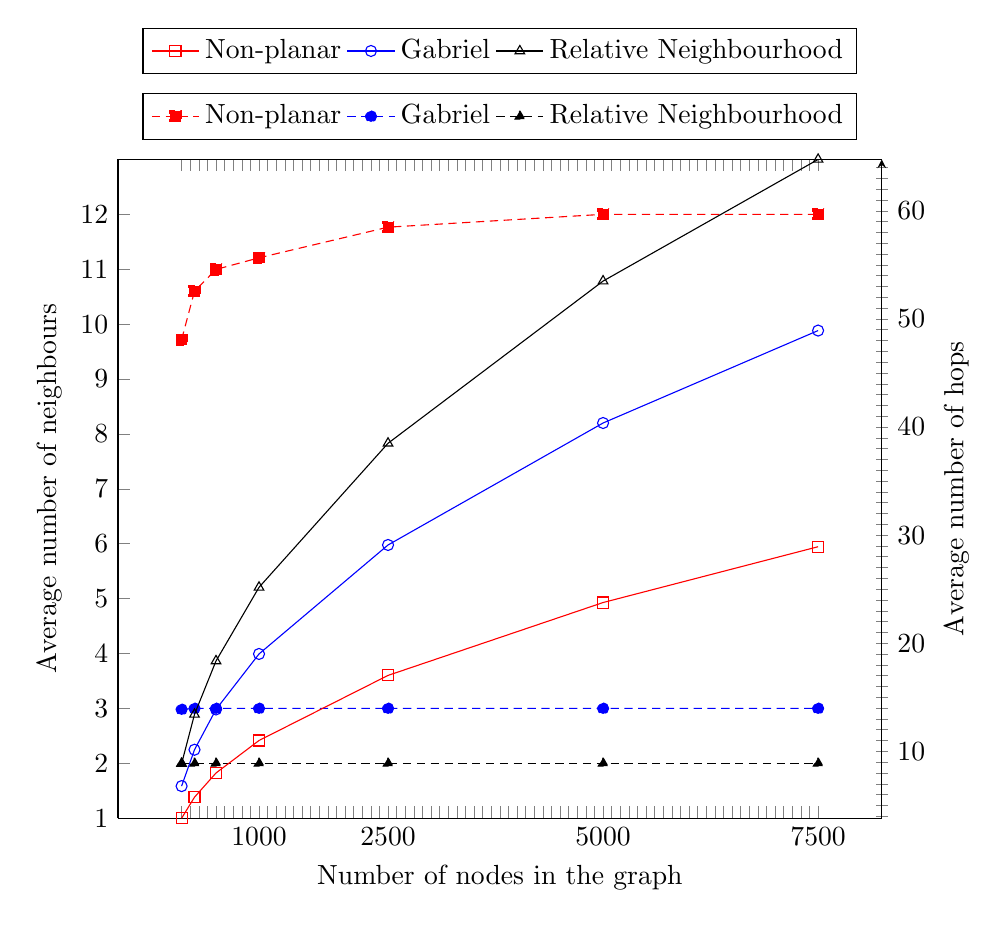
\begin{tikzpicture}
\pgfplotsset{every axis legend/.append style={at={(0.5,1.03)},anchor=south}, }
\begin{axis}[scale only axis, xtick={100, 200, 300, 400, 500, 600, 700, 800, 900, 1000, 1100, 1200, 1300, 1400, 1500, 1600, 1700, 1800, 1900, 2000, 2100, 2200, 2300, 2400, 2500, 2600, 2700, 2800, 2900, 3000, 3100, 3200, 3300, 3400, 3500, 3600, 3700, 3800, 3900, 4000, 4100, 4200, 4300, 4400, 4500, 4600, 4700, 4800, 4900, 5000, 5100, 5200, 5300, 5400, 5500, 5600, 5700, 5800, 5900, 6000, 6100, 6200, 6300, 6400, 6500, 6600, 6700, 6800, 6900, 7000, 7100, 7200, 7300, 7400, 7500}, xticklabels={, , , , , , , , , $1000$, , , , , , , , , , , , , , , $2500$, , , , , , , , , , , , , , , , , , , , , , , , , $5000$, , , , , , , , , , , , , , , , , , , , , , , , , $7500$}, ytick={1,...,12}, yticklabels={1,...,12}, legend columns=4,width=0.8\linewidth, axis y line*=left, xlabel=Number of nodes in the graph, ylabel=Average number of neighbours]
\addplot[color=red, mark=square*, densely dashed] coordinates{
	(100, 9.718)
	(250, 10.6)
	(500, 10.996)
	(1000, 11.208)
	(2500, 11.766)
	(5000, 12.0)
	(7500, 12.0)
};
\addplot[color=blue, mark=*, densely dashed] coordinates{
	(100, 2.982)
	(250, 3.0)
	(500, 3.0)
	(1000, 3.0)
	(2500, 3.0)
	(5000, 3.0)
	(7500, 3.0)
};
\addplot[color=black, mark=triangle*, densely dashed] coordinates{
	(100, 2.0)
	(250, 2.0)
	(500, 2.0)
	(1000, 2.0)
	(2500, 2.0)
	(5000, 2.0)
	(7500, 2.0)
};
\legend{Non-planar, Gabriel, Relative Neighbourhood}
\end{axis}

\pgfplotsset{every axis legend/.append style={at={(0.5,1.20)},anchor=north}}
\begin{axis}[scale only axis, ytick={1, 2, 3, 4, 5, 6, 7, 8, 9, 10, 11, 12, 13, 14, 15, 16, 17, 18, 19, 20, 21, 22, 23, 24, 25, 26, 27, 28, 29, 30, 31, 32, 33, 34, 35, 36, 37, 38, 39, 40, 41, 42, 43, 44, 45, 46, 47, 48, 49, 50, 51, 52, 53, 54, 55, 56, 57, 58, 59, 60, 61, 62, 63, 64, 65, 66}, yticklabels={, , , , , , , , , $10$, , , , , , , , , , $20$, , , , , , , , , , $30$, , , , , , , , , , $40$, , , , , , , , , , $50$, , , , , , , , , , $60$, , , , , , }, width=0.8\linewidth, legend columns=4, axis y line=right, axis x line=none, ylabel=Average number of hops]
\addplot[color=red, mark=square] coordinates{                
	(100, 3.81374)
	(250, 5.759968)
	(500, 7.99734)
	(1000, 11.004504)
	(2500, 17.024644)
	(5000, 23.765384)
	(7500, 28.92944)
};
\addplot[color=blue, mark=o] coordinates{                
	(100, 6.784)
	(250, 10.14888)
	(500, 13.877536)
	(1000, 19.008874)
	(2500, 29.09024)
	(5000, 40.3726888)
	(7500, 48.9245866667)
};
\addplot[color=black, mark=triangle] coordinates{                
	(100, 8.8698)
	(250, 13.419864)
	(500, 18.360056)
	(1000, 25.173018)
	(2500, 38.4983472)
	(5000, 53.5018848)
	(7500, 64.7559082667)
};
\legend{Non-planar, Gabriel, Relative Neighbourhood}
\end{axis}
\end{tikzpicture}
